\subsection{Результаты моделирования}
Результаты решения системы в безразмерных единицах при типичных условиях представлены на~\autoref{pic::Model::results::Te-200eV_ne-1e13cm^-3}. 
Полученные значения согласуются с классическими~\cite{hobbs1967heat} при малых значениях $T_s$: $V_f \approx -2.7$.

Наибольший интерес представляет тот факт, что при переходе в режим экранирования объёмным зарядом, ток термоэлектронной эмиссии 
идеально экранируется виртуальным катодом. Значение потенциала виртуального катода постоянно при изменении температуры, 
плавающий потенциал линейно растёт при увеличении температуры поверхности плитки.

Уменьшение $\varphi_{se}$ с ростом температуры $T_s$ соответствует увеличению потока ионов на плитку. Приращение потока термоэлектронной эмиссии 
приводит к эффективному росту плавающего потенциала $V_f$. Согласно~\eqref{eq::quasineutral_j_balance} и~\eqref{eq::j_sum_classic}:
\begin{equation}
    j_e \propto \exp{\left\{{V_f}\right\}} \propto \sqrt{\cfrac{2\pi m_e}{m_i}}\cfrac{n_i^{se}}{n_e^{se}} + \cfrac{j_s}{\cfrac{1}{4}en_e^{se}\upsilon_e^{th}} 
\end{equation}

\hl{В общем случае, $n_e^{se} \slashed{\propto} j_s$, что приводит к тому, что рост термоэлектронной эмиссии не обязан быть полностью скомпенсированным 
пропорциональным увеличением потока электронов из плазмы. Однако, при фиксированном $\varphi_{se}$ решение системы с исключенным для устранения 
переопределенности критерием Бома возможно, что и будет применено далее.}

По полученному решению построен график зависимости $q(T_s)$~\autoref{pic::Model::results::q_Te-200eV_ne-1e13cm^-3}. При малых температурах тепловой поток 
согласуется с классическим результатом~\cite{stangeby2000plasma}

Распределение потенциала в дебаевском слое может быть получено решением уравнения Пуассона в слое. 
На~\autoref{pic::Model::results::Poisson_Te-200eV_ne-1e13cm^-3} приведено решение для режима объёмного экранирования. Разность потенциалов 
между поверхностью стенки и виртуальным катодом является величиной порядка $T_s - T_{trans}$.

\begin{figure}[H]
	\centering
	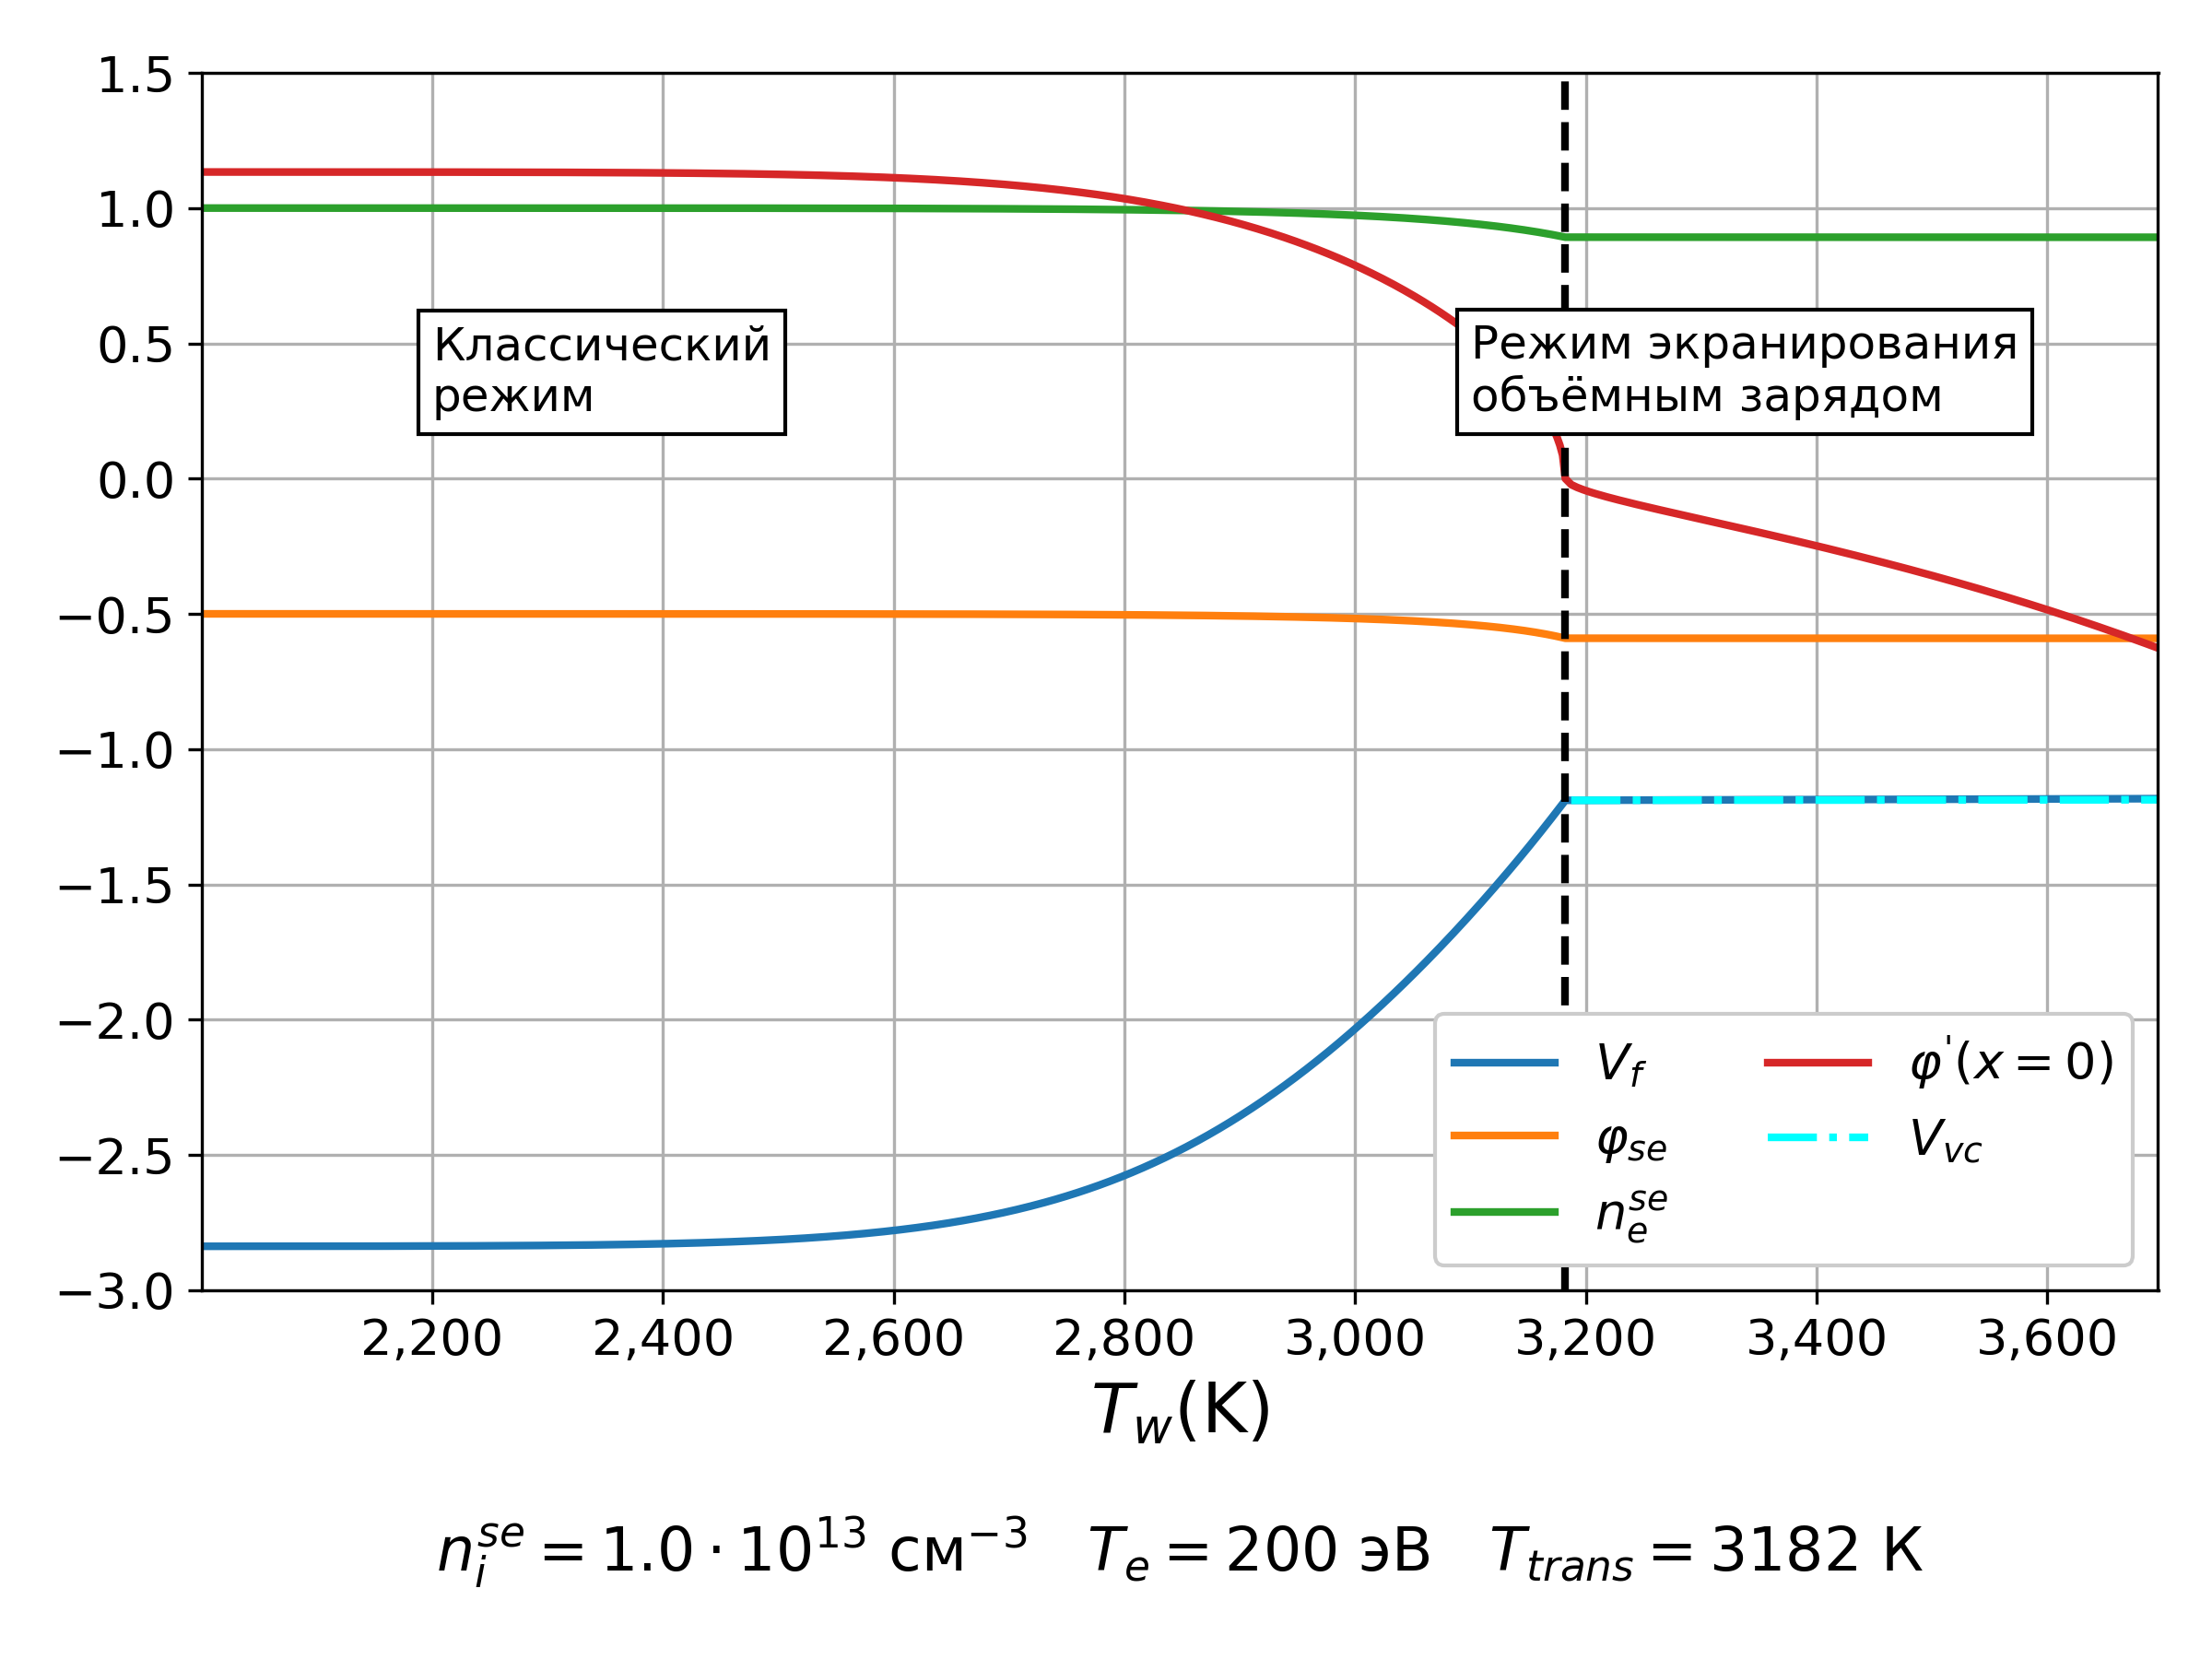
\includegraphics[width=0.7\linewidth]{material/Te=200eV_nse=1.0e13.png}
    \caption[]{График решения систем для поиска параметров дебаевского слоя при заданных $n_i^{se}, T_s$}
	\label{pic::Model::results::Te-200eV_ne-1e13cm^-3}
\end{figure}

\begin{figure}[H]
	\centering
	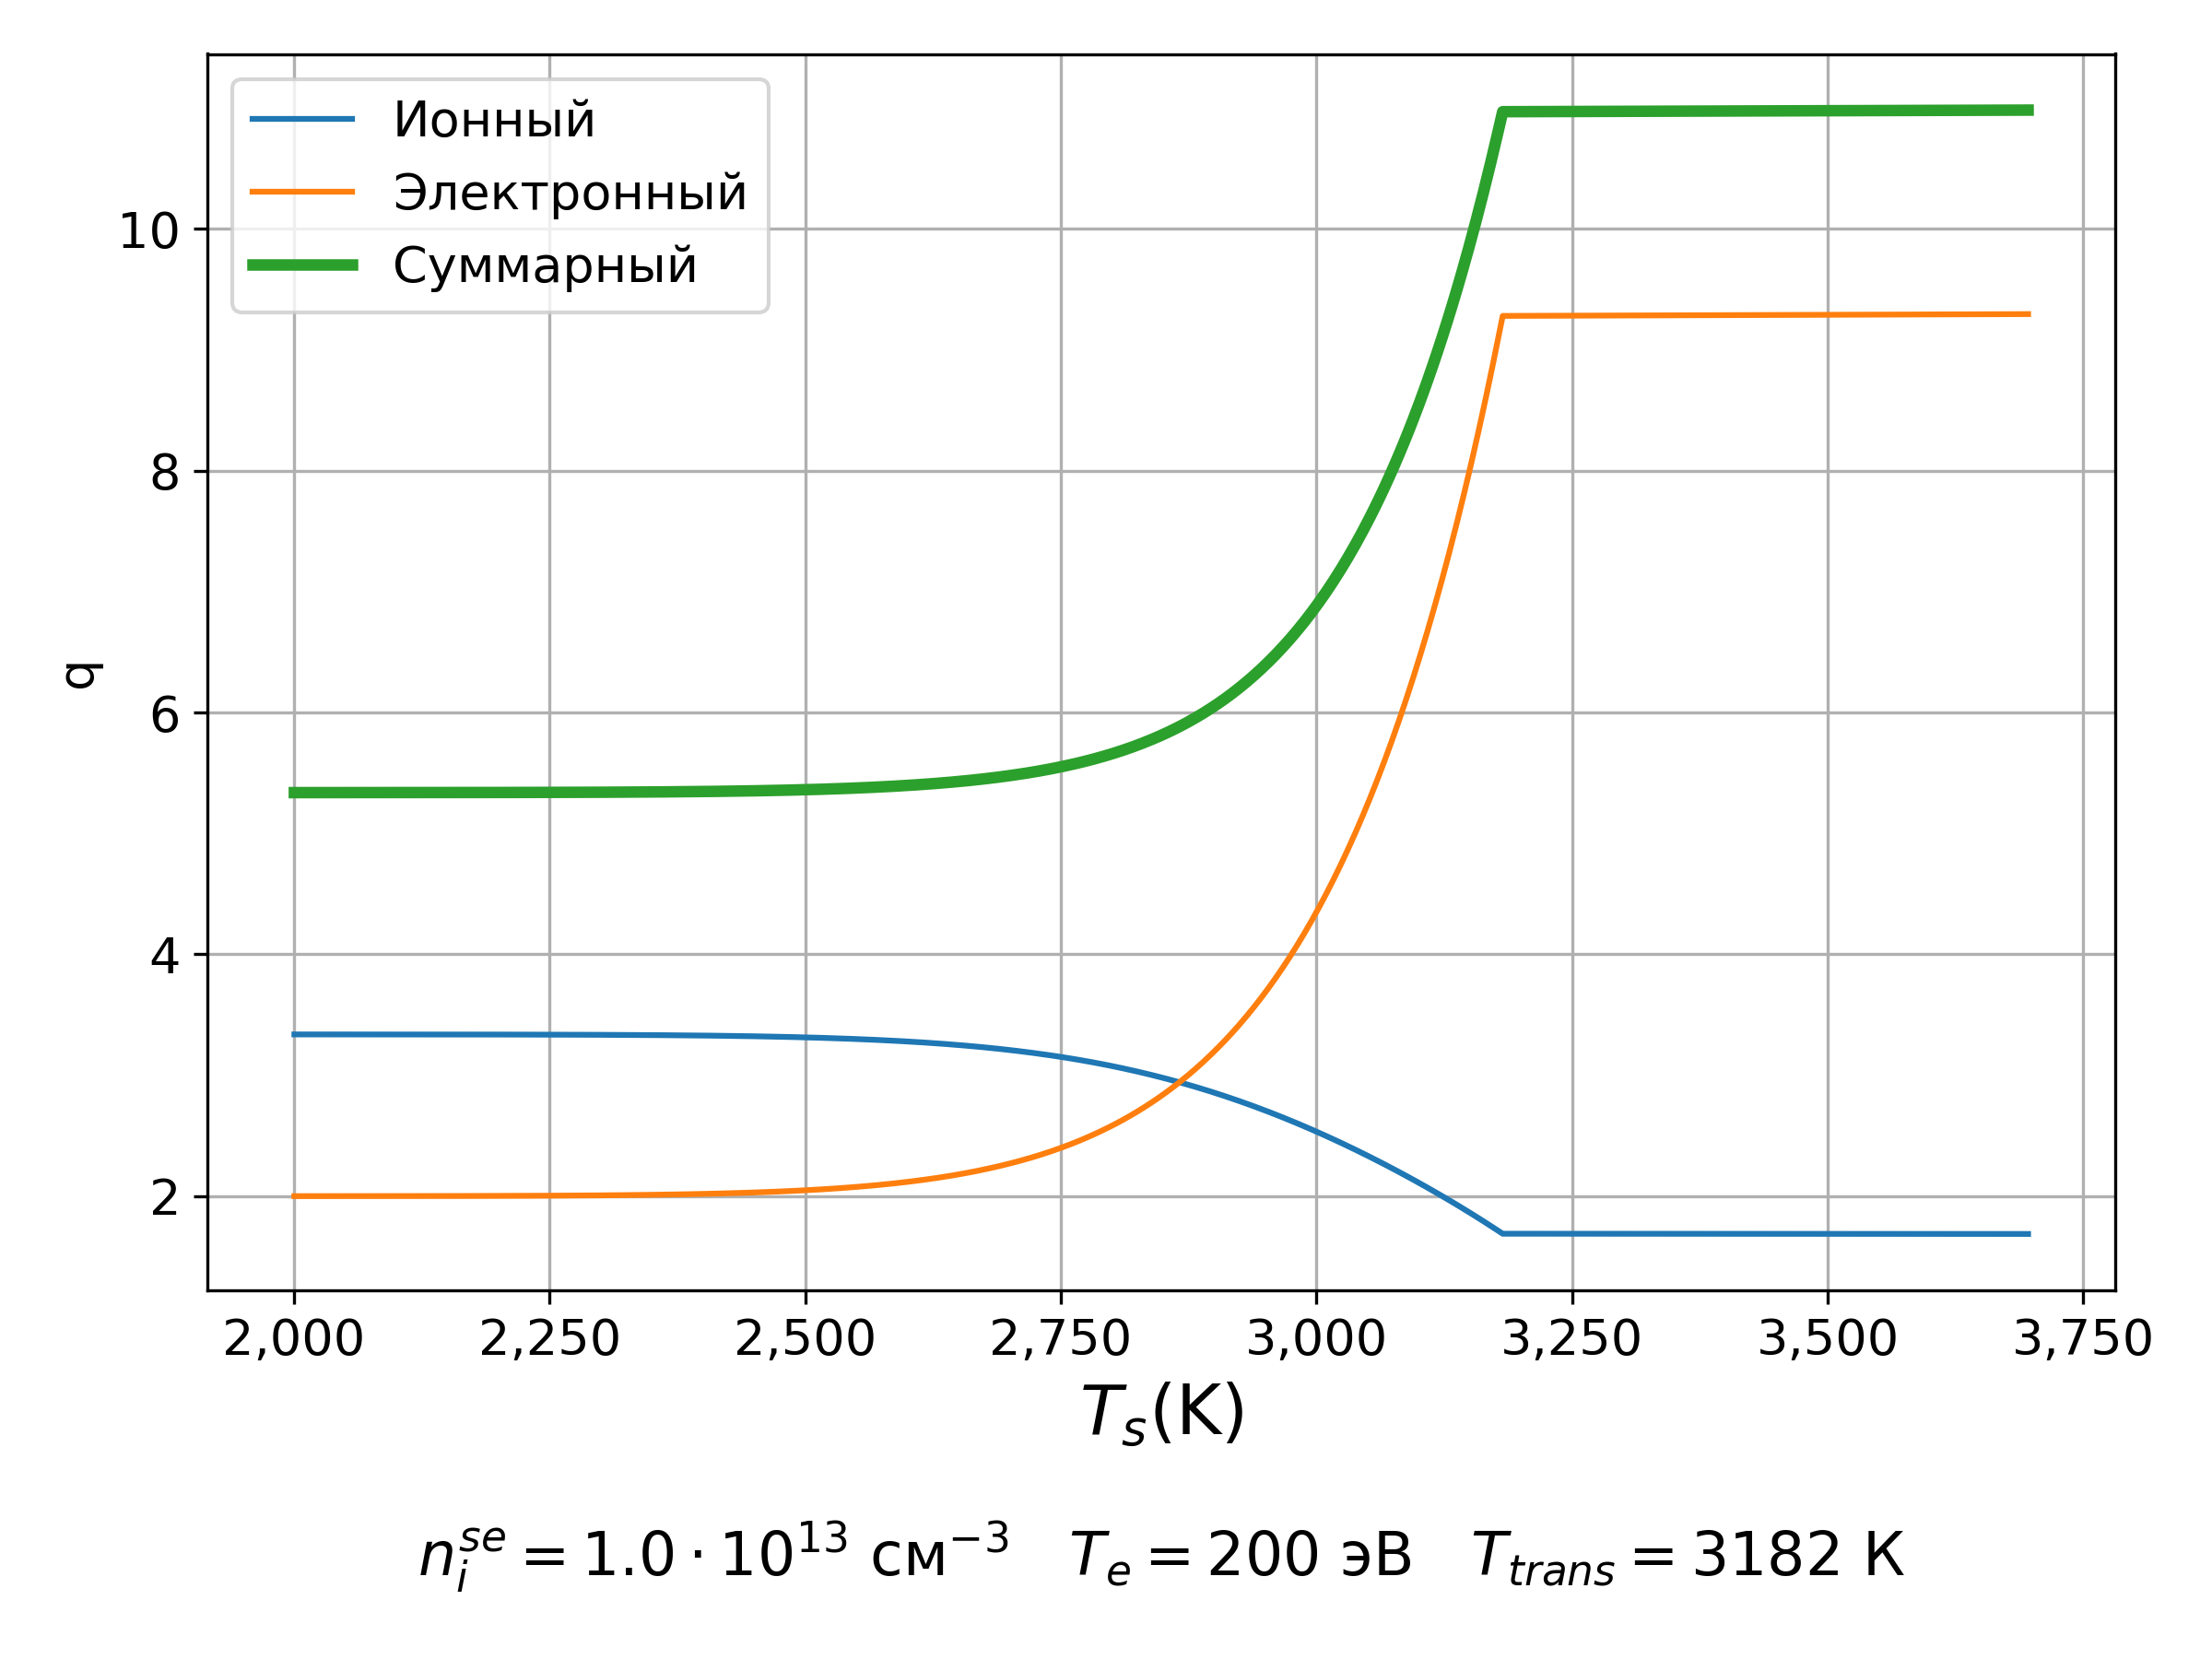
\includegraphics[width=0.7\linewidth]{material/q_plot_Te=200eV_nse=1.0e13.png}
    \caption[]{График зависимости теплового потока от температуры поверхности плитки}
	\label{pic::Model::results::q_Te-200eV_ne-1e13cm^-3}
\end{figure}

\begin{figure}[H]
	\centering
	\begin{subfigure}{\textwidth}
		\centering
	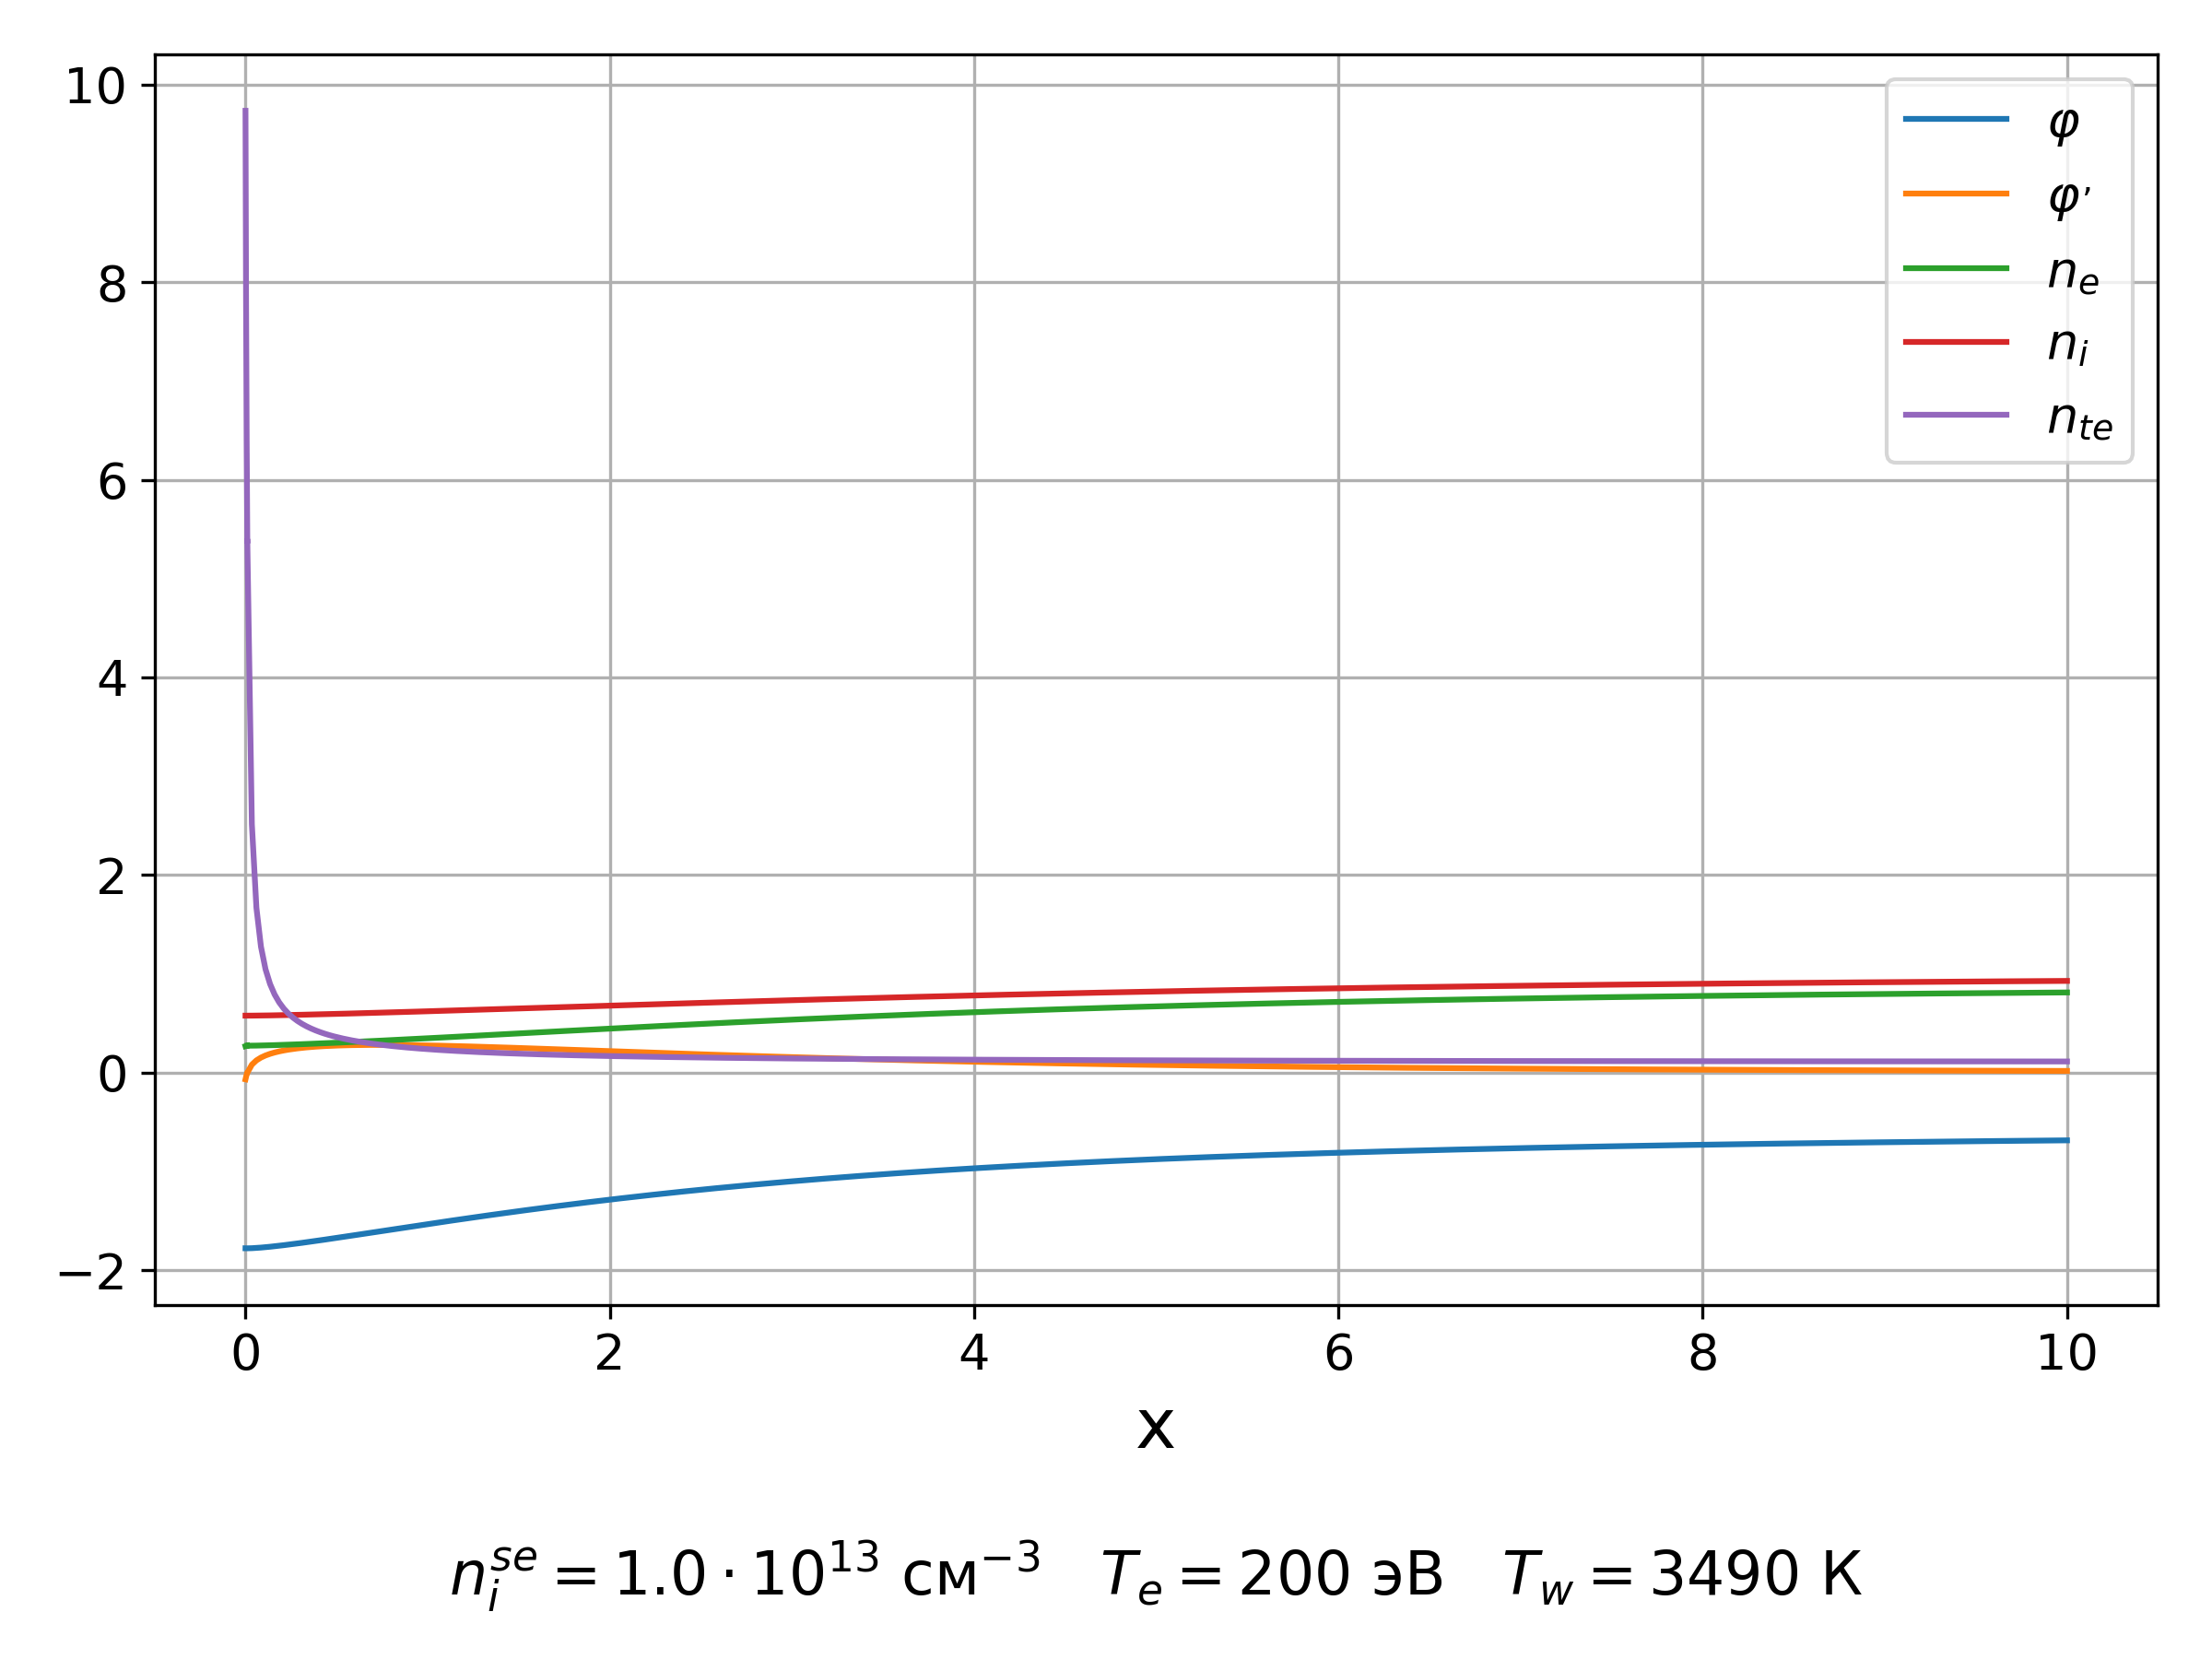
\includegraphics[width=0.7\linewidth]{material/plot_Te=200eV_nse=1.0e13.png}
    \caption[]{В области между поверхностью плитки и входом в дебаевский слой}
	  \end{subfigure}%
    \hfill
	\begin{subfigure}{\textwidth}
	  \centering
        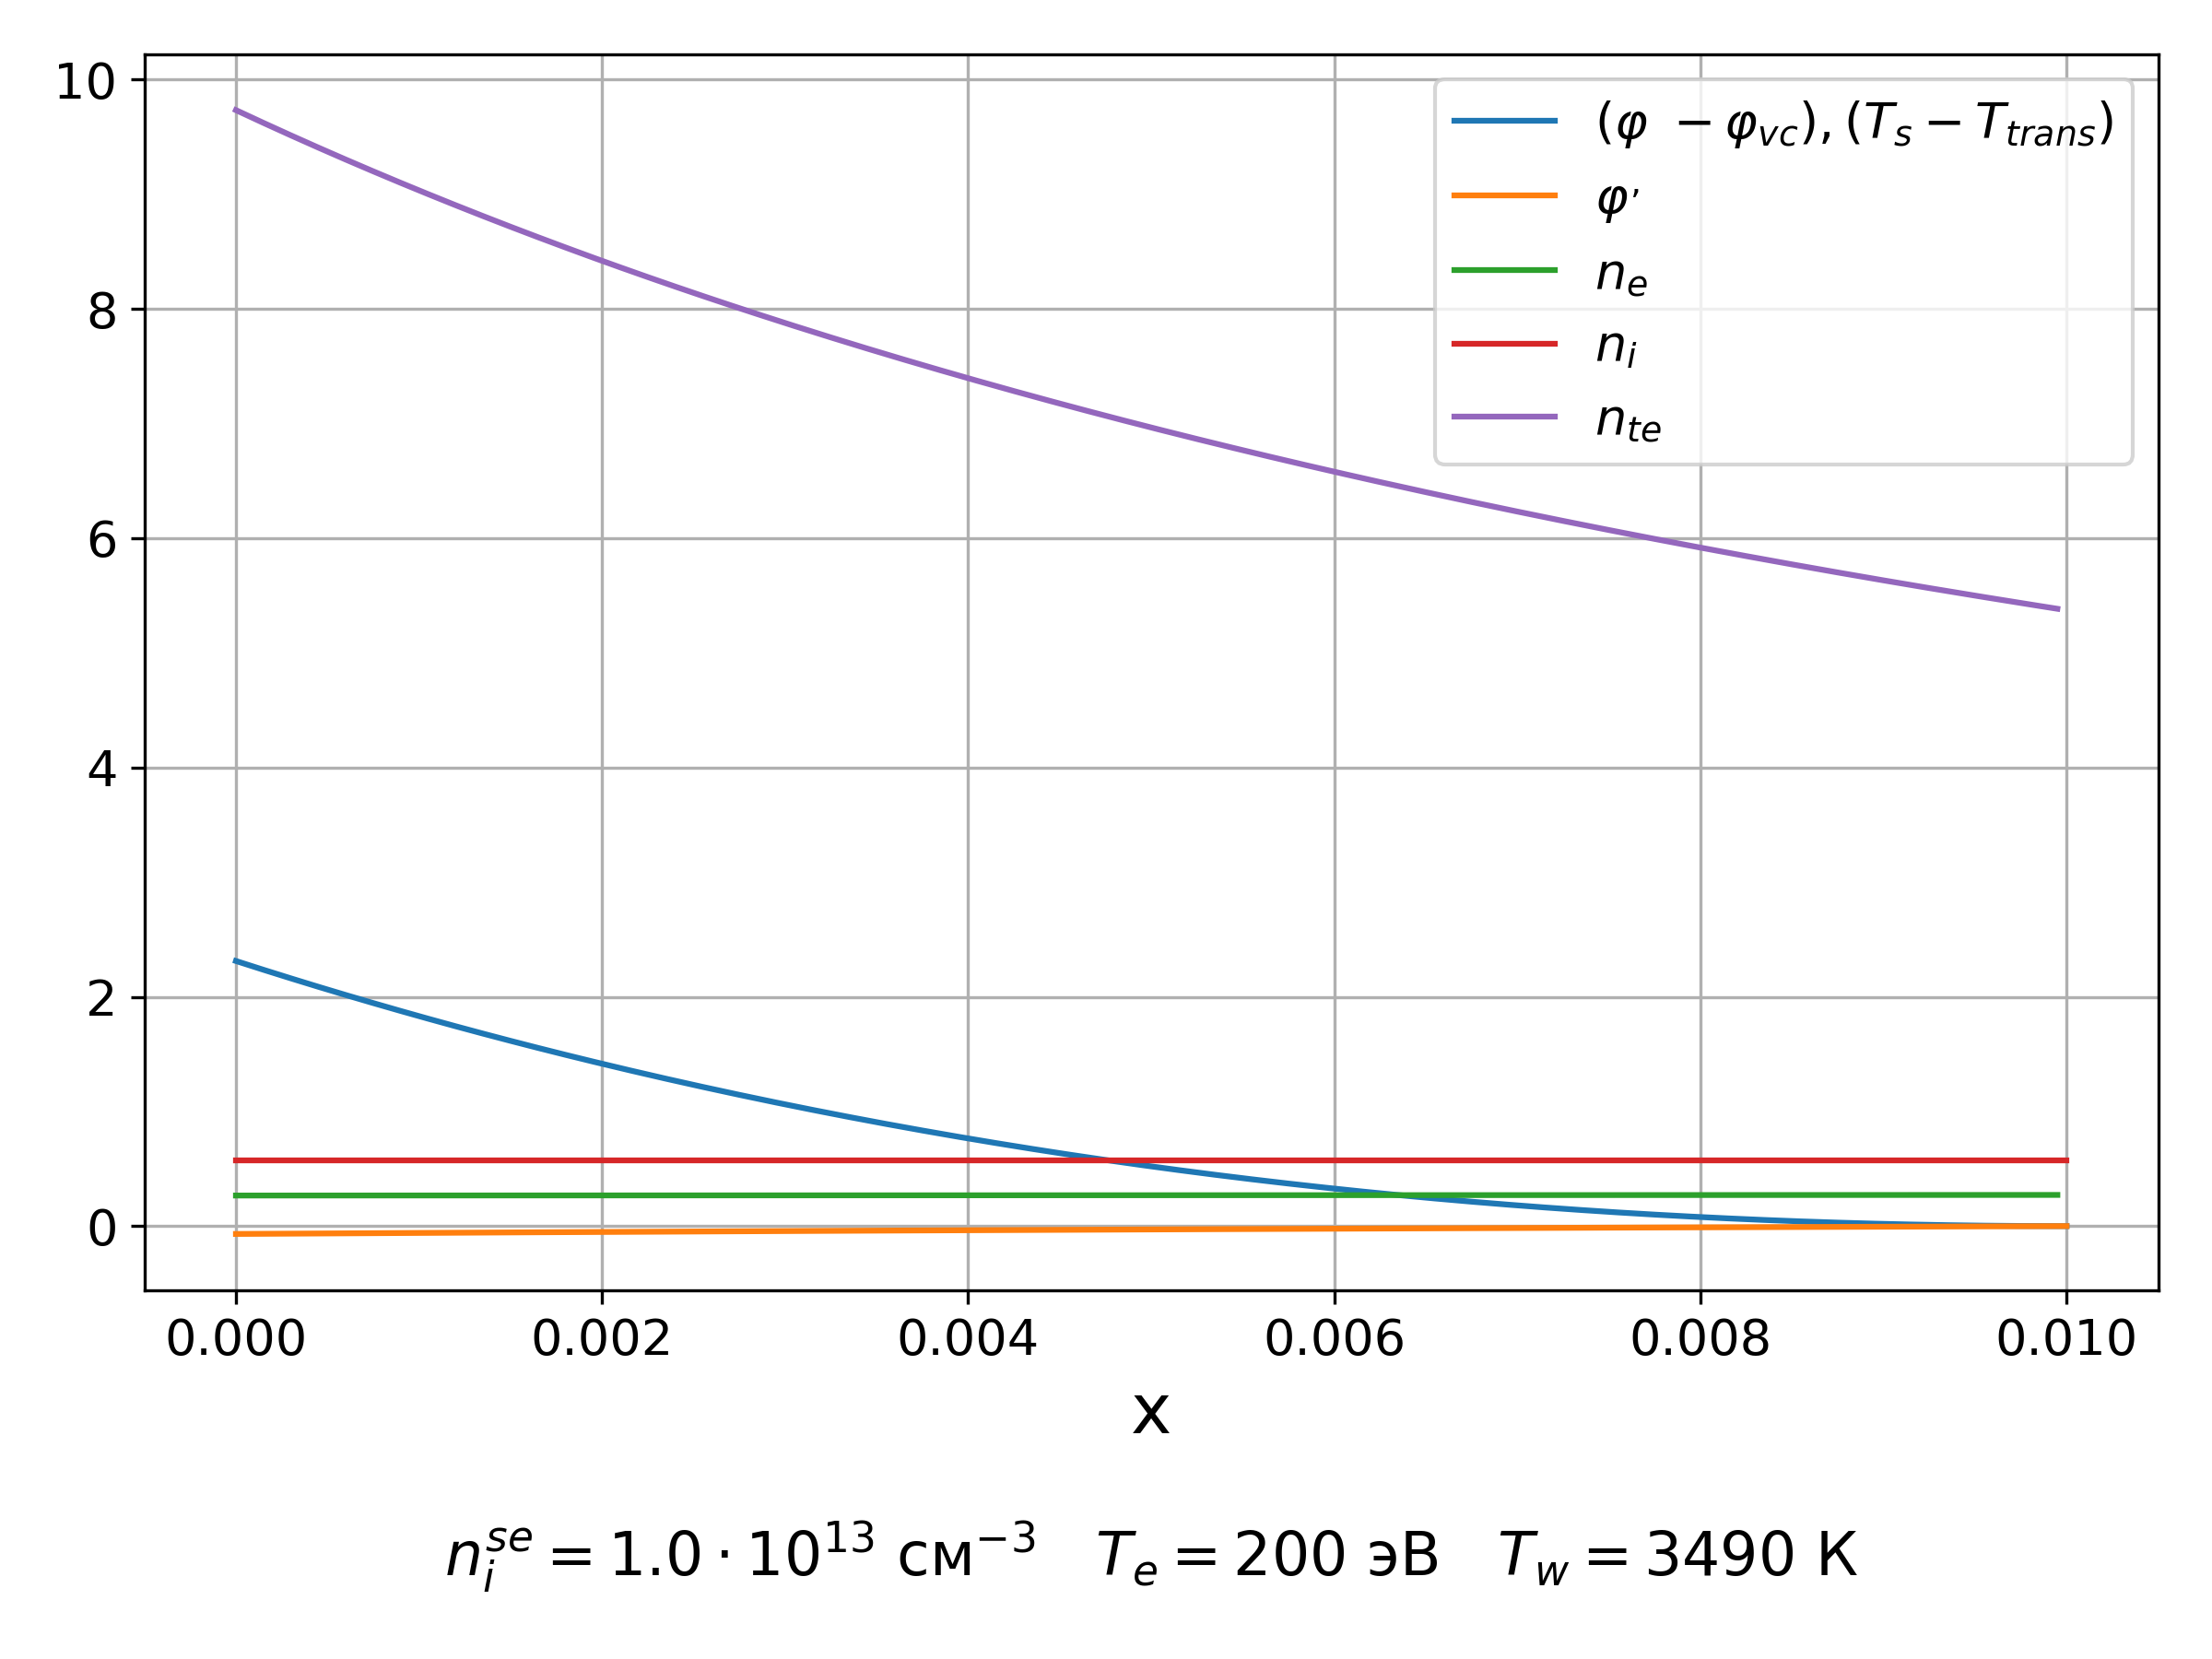
\includegraphics[width=0.7\linewidth]{material/plot_alpha_Te=200eV_nse=1.0e13.png}
    \caption[]{В области между поверхностью плитки и виртуальным катодом}
	\end{subfigure}%
    \caption[]{Графики решений уравнения Пуассона в режиме объёмного экранирования зарядом}
	\label{pic::Model::results::Poisson_Te-200eV_ne-1e13cm^-3}
\end{figure}
\clearpage
